\subsection{Operational setting for \proj}

Off shore in the \naz canyon-Berlengas area are two islands of
Berlengas and Farilho\~es part of a protected nature preserve. With
special permission we expect to be able to be based in Berlengas for a
period of 3 weeks to conduct off shore operations. A small team will
also be present onboard the 70 m \inst research vessel
(Fig. \ref{fig:vessel}) where if needed, deployment and recovery of
assets well off shore at the boundaries of the survey region, can be
done. In addition \inst will be in a position to provide a RHIB or a
rigid boat for near-shore operations from the two islands. \univ will
provide the bulk of the robotic assets including aerial, surface and
underwater vehicles as also the team to operate them. The team will be
split between being based in Berlengas, the research vessel and also
provide remote monitoring from Porto. \soc will provide at least one
glider to operate outside the shelf to augment model observations in
the meso-scale. For operational safety the gliders will operate
outside the maritime shipping zone in the blue-shaded region in
Fig. \ref{fig:domain}.

\proj will leverage existing real-time monitoring capacities which
were installed and are operated by Instituto Hidrogr\'{a}fico
(\inste). These include two multi-parametric buoys with satellite
transmission of hourly data sets and two coastal tide gauges installed
in the ports of \naz and Peniche. These systems form the \naz Canyon
Observatory which is a subset of the global real-time monitoring
infrastructure for the Portuguese Exclusive Economic Zone operated by
\inst (Fig. \ref{fig:po-map}). In addition, we will leverage ship time
from one of the \inst research vessels which visit the \naz area for
buoy maintenance twice yearly. \inst will provide access to this
vessel where a small \proj team will be resident, in addition to those
being housed in the Berlengas island.

Each multiparametric buoy is equipped with:

\begin{enumerate}[noitemsep,topsep=0pt,parsep=0pt,partopsep=0pt]

  \item A meteorological mast providing hourly measurements of wind speed and
    direction, air temperature, atmospheric pressure and relative
    humidity

  \item A wave sensor providing hourly measurements of standard wave parameters
    (wave spectra at the end of the deployment)

  \item A downward looking 300 kHz RDI Workhorse ADCP installed at 7 m
    depth and providing currents with $sim 2$ m resolution to about 90 m
    depth Surface temperature sensor (SBE AADI Subsurface temperature
    sensors)

\end{enumerate}  


The buoys are also equipped with fluorometers but the response of these
sensors rapidly degrades in about 1-2 weeks, after maintenance,
primarily due to biofouling.

Additional systems could also be available for \proj such as % . A separate
% project proposal was submitted at the end of 2020~\footnote{EEA Grants,
%   Portugal} where 
a HF radar system has been proposed for the \naz area. The system, a
CODAR Seasonde with two antennas operating at 13 MHz, one installed in
\naz and the other in Peniche. A previous test of a similar system was
conducted by \inst in September--November 2011 and showed that surface
currents measurements were available for the complete area to about 70
km from the shore with a 1 km resolution.

\soc will carry out a glider mission using one Slocum glider in the
\naz Canyon to understand the boundary conditions and off-shore waters
being entrained into the region. % SOCIB will be responsible for the
% glider launching, piloting, recovery of the glider, and evaluating the
% glider observations together with Fresnel scientists and
% technicians. The glider preparations will be taking place at the IH
% laboratory facilities.
Gliders are complementary to powered AUVs, providing significantly
greater range and endurance, and allowing repeated monitoring of sections
to capture spatial and temporal variability. % Missions can at present
% extend from days to several months and can cover thousands of
% kilometers of range.
% The glider can dive from the surface to up to
% 1000 m for months following a programmed trajectory, allowing
% scientists to observe the study area monitoring mesoscale and
% submesoscale features repeatedly. The typical up-and-down,
% sawtooth-like profile followed by a glider can provide data on
% different temporal and spatial scales unattainable by powered AUVs and
% much more costly to sample using traditional shipboard techniques.
The \soc glider will carry a suite of physical and biochemical sensors
that will make measurements including temperature, conductivity,
surface and depth average currents, chlorophyll fluorescence, and
optical backscatter. The glider observations will augment other
robotic platform observations and provide insight into physical and
biogeochemical processes for the marine ecosystem in
\naze. % that scientists might not otherwise
% be able to detect from satellites and ship-based observations.

  
\subsection{At-Sea operations}

\proj will observe the coastal ocean area of interest off of \naze, in
such a way as to improve the initialization/assimilation fields and
parameter definitions to be used in the physical and biogeochemical
models. To achieve this objective \proj will develop a strategy
largely inspired in the strategies used during the Rapid Environmental
Assessment to Navy operations. A summary of roles, tasks and
activities of different elements in the project is summarized in Table
\ref{tab:tasks}. A total of three phases (weeks 1 to 3) are planned:

\begin{figure}[!t]
  \vspace{-0.5cm}
  \centering
  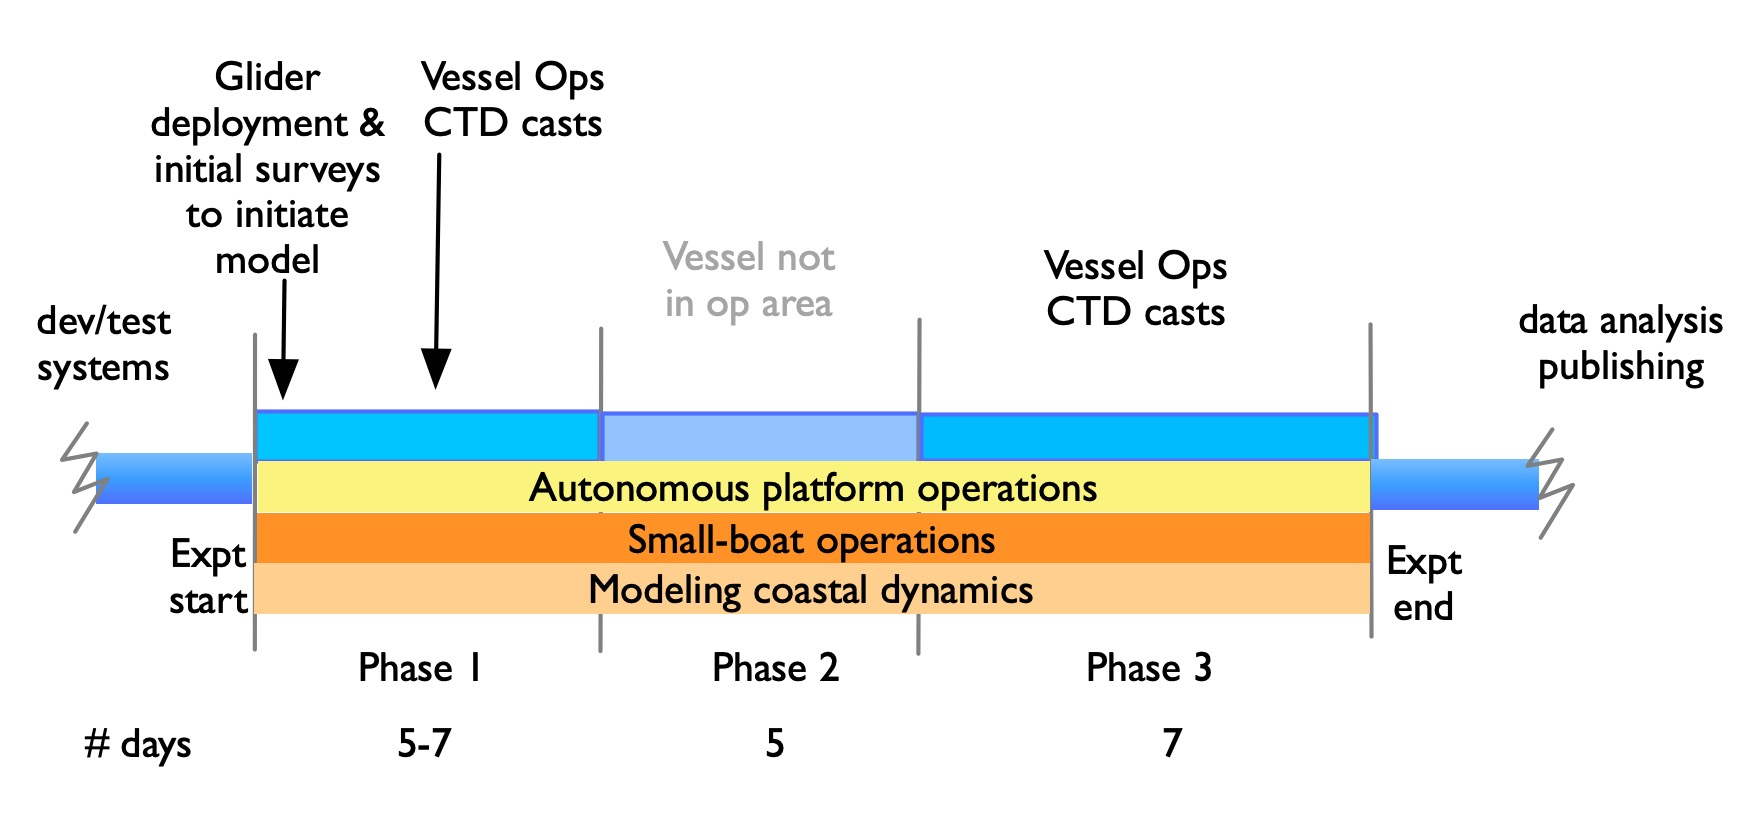
\includegraphics[scale=0.25]{fig/timelines.jpg}
  \caption{At-sea operations for \proj will be split along 3 phases.
    Phase 1 will involve glider deployments at the further reaches of
    the operational boundary, deployment of other autonomous platforms
    to initialize the model, calibrate sensors with limited ship based
    CTD casts. Phase 2 will commence when the vessel departs the \naz
    operational area. Phase 3 will commence with the resumption of
    vessel ops in the \naz area. Autonomous platforms starting with
    gliders will be operating continuously to target adaptive sampling
    driven by model predicts, through all phases.}
  \vspace{-0.3cm}
 \label{fig:expt-phases}
\end{figure}

 
% Phase 1 (precursor survey):
\paragraph{Phase 1} A preliminary characterization of the geographical
area of interest will be conducted during this phase with the
identification of the prevailing features that characterize the coastal
ocean area of \naz from remote sensing imagery and (if available) from
surface currents measured by HF radar. The data will allow
identification in SST, Chl, turbidity and currents, for example, and to
select a limited number of key stations which can be complemented by CTD
casts. % In case no surface data is
% available (because of cloud cover obstructing optical remote sensing)
% the location of these points will be dictated by the characteristics of
% the topography of the area, by the prevailing forcing conditions and by
% previous knowledge about the primary processes.
This phase will combine operations from small boats with operations
conducted onboard a \inst hydrographic vessel that will pass through the
area. Glider deployments off-shore to provide boundary conditions for
the models will be initiated and augment available remote sensing (or HF
radar) data. Sampling with vertical nets will also be done at some
stations; part of the water samples collected will be used to evaluate
the nutrient profiles in the water column. % These samples will be
% analyzed at the \inst Marine Chemistry and Pollution laboratories and
% will be available in about 1--2 days.
They will aid in characterizing the nutrient intake to upper levels
associated with intensified upwelling at the canyon head or the inputs
to the coastal ocean associated by freshwater inputs along the coast as
a means to initialize the nutrient fields in the BGC model. Analysis of
water samples collected by the small boats will be used for calibration
of the CTD fluorometer and as also to calibrate the ADCP echo intensity
data for zooplankton biomass. Remote operations from Porto will also be
tested as a means to demonstrate an Ocean Space Center (OSC)
\cite{lima21}. This phase will likely be between 5--7 days.

% During 2--3 days a team onboard a small-boat will conduct a set of
% measurements in the water column (to about 200 m depth) at the key
% location point identified earlier using low cost systems \kc{this is
%   vague} and other sensors of interest and water samples collected at
% selected depths on those key locations. Sampling with vertical nets will
% also be done at some of these positions. Part of the water samples
% collected will be used to evaluate the nutrient profiles in the water
% column. These samples will be analyzed at the \inst Marine Chemistry and
% Pollution laboratories and will be available in about 1--2 days.
% Depending on the period selected for the exercise these measurements
% would help to characterize the nutrient intake to upper levels
% associated with intensified upwelling at the canyon head or the inputs
% to the coastal ocean associated by freshwater inputs along the coast.
% Combined with the information available from remote sensing images, this
% data will provide the basis for the initialization of the nutrients
% fields in the BGC model.
 
% Part of the water samples and samples collected with a vertical net will
% be used to characterize the phyto- and zoo plankton communities. These
% samples will provide the basis for the initialization of the phyto and
% zooplankton compartments of the BGC model.
 
% At the same time the hydrographic vessel will pass on the area and
% during this period will conduct a very limited number of CTD profiles
% and collect vessel mounted ADCP measurements. The analysis of water
% samples collected by the small boat campaign at a few locations and same
% times will then be used for calibration of the CTD fluorometer and
% calibrate the ADCP echo intensity data in zooplankton biomass. These
% calibrations will then be used during next phase of the survey

% \kc{
% This data will also be used to calibrate the response of fluorometers to
% be used in response
 
% This phase will provide key points to be used in the following stages
% such as vertical profiles of temperature and salinity and water samples
% collected at selected depths to be used in the definitions of d
% will be inspired in the strategies used with real and assimilation
% fields. In \proj we propose to extend this This phase will provide the
% background knowledge to be used in the numerical model initialization
% such as and the definition of some of the basic parameters (such as
% light attenuation parameters and so one).. Also during this phase we
% calibrate the response of the some of the sensors using}

\paragraph{Phase 2} This phase will rely only on small boat operations
with the departure of the research vessel and provide additional
opportunities to fine tune the adaptive sampling algorithms, model
predictions and BGC model fields. Glider operations will continue to
provide updates to boundary conditions in the model even as other
autonomous platforms will continue to operate in a more constrained
field of scientific interest. Small boat operations will be from
Berlengas or \naz itself, especially for launch and recovery operations.
Monitoring autonomous platforms from remote shore-side locations will
continue. This phase will likely be around 5 days and contingent on the
research vessel being able to complete its buoy maintenance tasks north
of the \naz operational area.

\paragraph{Phase 3} This phase will commence when the research vessel
returns to the \naz operational area for exclusive use of \proje, and
will result in intense operation of all assets and personnel. Repeated
CTD casts to ground-truth model predictions, and the implementation of
the adaptive sampling algorithms will ensue. It is expected that results
from the lab analysis of previously obtained water samples will aid and
augment the sampling and prediction process. All autonomous platforms,
including gliders, will continue continuous day-time operations. We will
consider night-time operations of powered AUVs, on the shelf subject to
local conditions and importance of data collection to fill any
outstanding gaps. Should those be feasible, the use of the OSC will
significantly aid operations and demonstrate the applicability of
networked robotic operations even in constrained near-shore locations.
This phase will last a full 5 days concentrating the efforts and energy
of all participants.

\paragraph{Post experiment} At the completion of the experiment and
demobilization, modeling the water-column will continue based on the
sampling from the prior weeks, primarily to demonstrate improvement with
assimilation. In this case the models will be run in hindcast mode to
give us the best possible description of evolution of conditions during
the two weeks of the experiment.


\begin{table}[!t]
  \centering
  % \vspace{-0.5cm}
  \footnotesize{
  \begin{tabular}{|p{4cm}|p{4cm}|p{4cm}|p{4cm}|}\hline 
    \rowcolor{Gray}
    \bfseries  &\bfseries Phase 1 &\bfseries Phase 2 &\bfseries Phase 3 \\
    \hline
    Main Goals& Precursor survey; To collect data to
                initialize fields and define model parameters,
                deployment and operations of autonomous vehicles. To
                calibrate sensor response& Update Survey 1: 
                                           AUV adaptive
                                           sampling operations;
                                           potential additional
                                           measurements using small boats
                                           and low cost measurements,
                                           model predictions to encapsulate
                                           high-res water-column surveys& Update Survey 2:
                                                                          Detailed
                                                                          ship
                                                                          measurements
                                                                          with
                                                                          dedicated
                                                                          surveys,
                                                                          continued
                                                                          autonomous system
                                                                          operations
                                                                          with
                                                                          adaptive
                                                                          sampling
                                                                          and
                                                                          model
                                                                          predictions\\
                                                                          % \hline
    \noalign{\hrule height 2pt}
    % Observations at sea&&&\\
    % \hline
    % AUVs&&&\\
    % \hline
    % Gliders&&&\\
    % \hline
    % UAVs&&&\\
    % \hline
    % ASVs&&&\\
    % \hline
   Autonomous vehicles (UAVs, AUVs, ASVs and Gliders)&Calibrate sensors
                                                        amongst all
                                                        assets incl.
                                                        research vessel
                                                        and sample in
                                                        proximity of
                                                        ID-ed key
                                                        stations.
                                                        Generated
                                                        (physical and
                                                        BGC) data
                                                        assimilated into
                                                        shore-side
                                                        models. Initiate
                                  adaptive sampling algorithms on
                                                        AUVs&Generate
                                                              science
                                                              data for
                                                              assimilation
                                                              into
                                                              models.
                                                              Onboard
                                                              embedded
                                                              tasking
                                                              for
                                                              adaptation
                                                              targeting
                                                              specific
                                                              variables
                                                              using
                                                              Gaussian
                                                              Processing
                                                              methods\cite{fossum19,fossum21},
                                                     provide hi-res
                                                              water-column
                                                     measurements&Generate
                                                                   data
                                                                   and
                                                                   adaptively
                                                                   control
                                                                   AUVs
                                                                   for
                                                                   hi-res
                                                                   water-column measurements\\
    \hline
    Models&Build initialization and initial assimilation fields. 
            Start model runs (end of the week). Generate model
            predictions (incl. BGC) based on assimilation of remote sensing and data
                                  from autonomous vehicles.&Generate model
            predictions (incl. BGC) based on assimilation of remote sensing and data
                                  from autonomous vehicles.&Generate model
            predictions (incl. BGC) based on assimilation of remote sensing and data
                                  from autonomous vehicles. Continue
                                                             work
                                                             post-cruise
    to refine hindcasts\\
    \hline
     Remote Sensing&SST, Chl, Turbidity images (Sentinel) used to
                    identify the main features and select key stattions for
                    observations. Surface fields combined with observations in key
                    stations to build initial 3D fields for models.&SST, Chl, altimetry data used in assimilation
                             Turbidity images used to track impacts (if
                             any) of local rivers and guide sampling
                                                                     strategy.
                                                     &SST, Chl,
                                                       altimetry data
                                                       used in
                                                       assimilation 
                                            Turbidity images used to
                                            track impacts (if any) of
                                            local rivers and guide
                                            observations.\\
    \hline
    Ship-based observations& Research vessel crosses the \naz op area, deploy Multi-parametric buoy
                             limited CTD casts, water sampling at key stations,
                             ADCP data collected at key stations&&CTD
                                                                   and
                                                                   ADCP profiles,
                                                                   rosette
                                                                   samples
                                                                   for
                                                                   nutrients/phyto/zoo-plankton
                                                                   ADCP on transit and at stations\\
    \hline
    Laboratory Analysis&Samples analyzed for Nutrients and
                         for phyto/zoo-plankton&Samples analyzed for Nutrients and
                         for phyto/zoo-plankton&Samples analyzed for Nutrients and
                         for phyto/zoo-plankton. Post cruise:
                                                  Samples analyzed to
                                                 enrich models for hindcasts\\
    \hline
    Small boat operations&CTD, fluorometry, profiles and samples at key
                           stations, for nutrients/phyto+zoo-plankton.
                           Vertical net samples for phyto/zoo-plankton&CTD, fluorometry, profiles and samples at key
                           stations&CTD, fluorometry, profiles and samples at key
                           stations\\
    \hline    
  \end{tabular}
  \caption{Summary of roles, tasks and activities with different assets
    and processes in \proj during Phases 1--3 (see Fig
    \ref{fig:expt-phases}).}
    \label{tab:tasks}
  }
\end{table}


\begin{wrapfigure}[17]{!h}{0.45\textwidth}
  \centering
  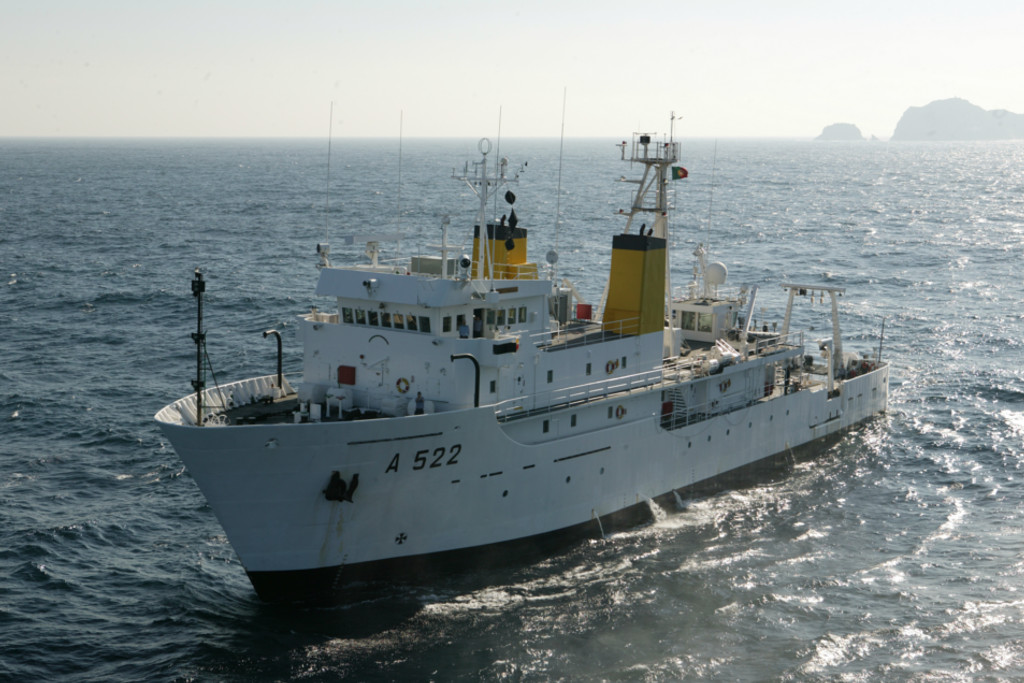
\includegraphics[scale=1.75]{fig/dom-carlos.jpg}
  \caption{A 70 m \inst research vessel, the NRP \emph{Dom Carlos} or
    its sister vessel will be available for \proje.}
  % \vspace{-1cm}
 \label{fig:vessel}
\end{wrapfigure}


\begin{figure}[!b]
  \centering 
  \subfigure[]{\label{fig:glider-1}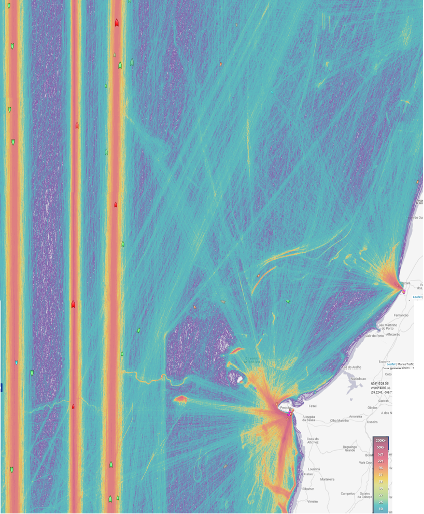
\includegraphics[scale=0.5]{fig/Nazare-traffic.png}}
  \hspace{+0.3cm} 
  \subfigure[]{\label{fig:glider-2}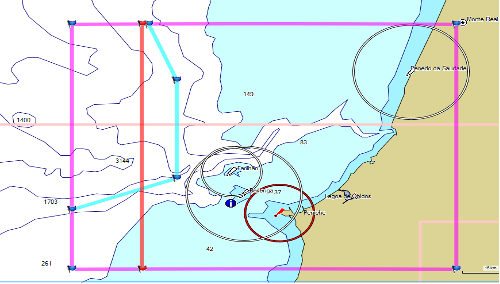
\includegraphics[scale=0.75]{fig/glider-lines.png}}
  \caption{Two possible \soc glider lines for
    deployment. \subref{fig:glider-1} indicates marked shipping
    lanes. The 5 mile gap between the western most and the next lane
    (in red) represents the volume at the model boundary. Operating
    the glider in Phase 1 of the experiment will be important to
    initialize boundary conditions. Subsequent movement of the glider
    line closer to the \naz canyon mouth in Phases 2 \& 3 shown in
    \subref{fig:glider-2} between the two (blue) flags, will capture
    the physical bio-geophysical couplings in the \naz canyon.}
  \label{fig:glider-ops}
\end{figure}


\paragraph{Operational Considerations} While most experiments in the
coastal zone rely on ship-board measurements and gliders, the
challenging nature of this high-energy environment requires a mix of
assets in addition to gliders. Currents can be in the region of
$\sim 2$ knots, there is substantial variability in the upper
water-column and with high primary productivity and the existence of
coastal upwelling to provide for a rich nutrient base and the study
region has a robust presence of fishermen, nets and crab pots. We
expect to field an ensemble of low cost robotic vehicles including
propelled AUVs, a glider, unmanned surface vehicles, low cost
Lagrangian profilers and aerial vehicles with RGB and potentially
hyper-spectral imaging sensors. 

The glider lines (Fig. \ref{fig:glider-ops}) will be critical to
initialize the boundary conditions in the model. One possible design
would be to have the glider to operate in Phase 1 between the two
shipping lanes on the far western edge of the model where the
separation between the lines is $\sim 5$ miles. In Phases 2 \& 3
considerations for the study of the bio-geophysical couplings could
move the line more inland east of the closest shipping lane
(Fig. \ref{fig:glider-2}). Typical sections will be $\sim 35$ km with
a daily coverage of $\sim 20-30$ km/day. While the glider can be
operated up to 1000 m depth to surface every 5-6 hours, we expect each
dive to be $\sim 300--500$ m to capture upper water-column dynamics to
aid the BGC models. 

Accessibility to the two islands will also provide some shelter from
weather for continuous operations including rapid launch/recovery of
in-situ assets. In addition, we will obtain images from the
\textbf{SeaHawk} nano-satellite (developed with funding from the Moore
Foundation when Subramaniam was program director there) with a high
quality multi-spectral
imager~\footnote{\url{https://uncw.edu/socon/index.html}}. Finally,
\univ and \inst have a number of low cost temperature/density sensors
which when calibrated with CTDs on the vessel and robotic vehicles,
will enable local fisherman to provide timely data in this meso-scale
region. All such data will be assimilated into the ocean models run by
\inst and supported by \mit which continues to support \texttt{HOPS}
development.

While our intent is to have the experiment in the September/October 2021
time frame, considering the current pandemic situation and the
associated uncertainties, we will have backup plans associated with the
following dates, which are coincident with when the \inst vessel visits
the \naz area for servicing buoys in that order:

\begin{itemize}[noitemsep,topsep=0pt,parsep=0pt,partopsep=0pt]
\vspace{+0.25cm}
\item Fall 2021 (Sept/Oct) -- primary target date
\item Spring 2022 (April/May)
\item Fall 2022 (Sept/Oct) 

\end{itemize}  

\paragraph{COVID protocol} As per standard oceanographic cruise
protocol in current circumstances, we will follow the guidance of WHO
and the US CDC; all personnel will isolate 5 days before the
experiment after appropriate PCR tests for safety and stay in one
pod. All US participants will be expected to be vaccinated prior to
the experiment with one of the European Medicines Agency-approved
vaccines. Those onboard the \inst research vessel will follow
Portuguese Navy guidelines and also isolate prior to the cruise and
have no contact with shore based personnel during the course of the
experiment.


\subsection{Current Pending Project and Proposal Submissions}

No proposals related to \proj have been submitted to any US government
agency. However, this proposal is in part to demonstrate a portion of
a much larger concept in the form of the \met project\footnote{See US
  National Academies 'Ocean Shot' presentation at
  \url{https://vimeo.com/510346249}} which is being proposed to
private philanthropies for funding. \met aims to provide a new
paradigm of portable coastal ocean observation using space, aerial,
surface and underwater vehicles, coupled to assimilative models.

\subsection{Relevant Experience}

% A description of the Offeror's Government contracts (both prime and
% major subcontracts) received during the past three (3) years, which
% are similar in nature to the effort being proposed.  Include contract
% number and the name, phone number and email address of the technical
% point of contact.  If necessary, add additional rows.

The PI and co-PI do not have any current US govt. contracts or have
had any US govt. contracts during the past 3 years.


